%%%%%%%%%%%%%%%%%%%%%%%%%%%%%%%%%%%%%%%%%%%%%%%%%%%%%%%%%%%%%%%%%%%%%%%%%%%%%%%%
%theory.tex: Chapter on light dark matter theory
%%%%%%%%%%%%%%%%%%%%%%%%%%%%%%%%%%%%%%%%%%%%%%%%%%%%%%%%%%%%%%%%%%%%%%%%%%%%%%%%
\chapter{Theoretical Framework}
\label{theory}
%%%%%%%%%%%%%%%%%%%%%%%%%%%%%%%%%%%%%%%%%%%%%%%%%%%%%%%%%%%%%%%%%%%%%%%%%%%%%%%%
There are two key aspects to the theory used in the search presented here: a model of a new physics which could produce dark matter used to simulate its interactions and determine our sensitivity, and a model of known physics, necessary to understand conventional processes which could mimic dark matter interactions as well as describe the initial states produced in the collision and the response of the detector to any produced particles.

The primary framework used to describe currently known particle physics is the standard model (SM), a quantum field theory which describes the set of known fundamental particles and their interactions.
In classical theories, particle interactions can be described via forces proportional to fields, such as the electromagnetic field applying a force directly proportional to the charge of a given particle.
In quantum field theories, particle interactions are instead described through the exchange of a gauge boson, allowing them to satisfy the requirements of special relativity and quantum physics. 
The SM contains five gauge bosons, which describe interactions with the nuclear strong, electroweak, and Higgs fields.
In addition, the SM includes six quarks, colored particles which can interact via the strong force, and six leptons, particles which only interact via the electroweak force.
A graphical representation of these fundamental particles is shown in \Cref{fig:SM}, along with numerical values of some of their physical properties.

\begin{figure}[htpb]
	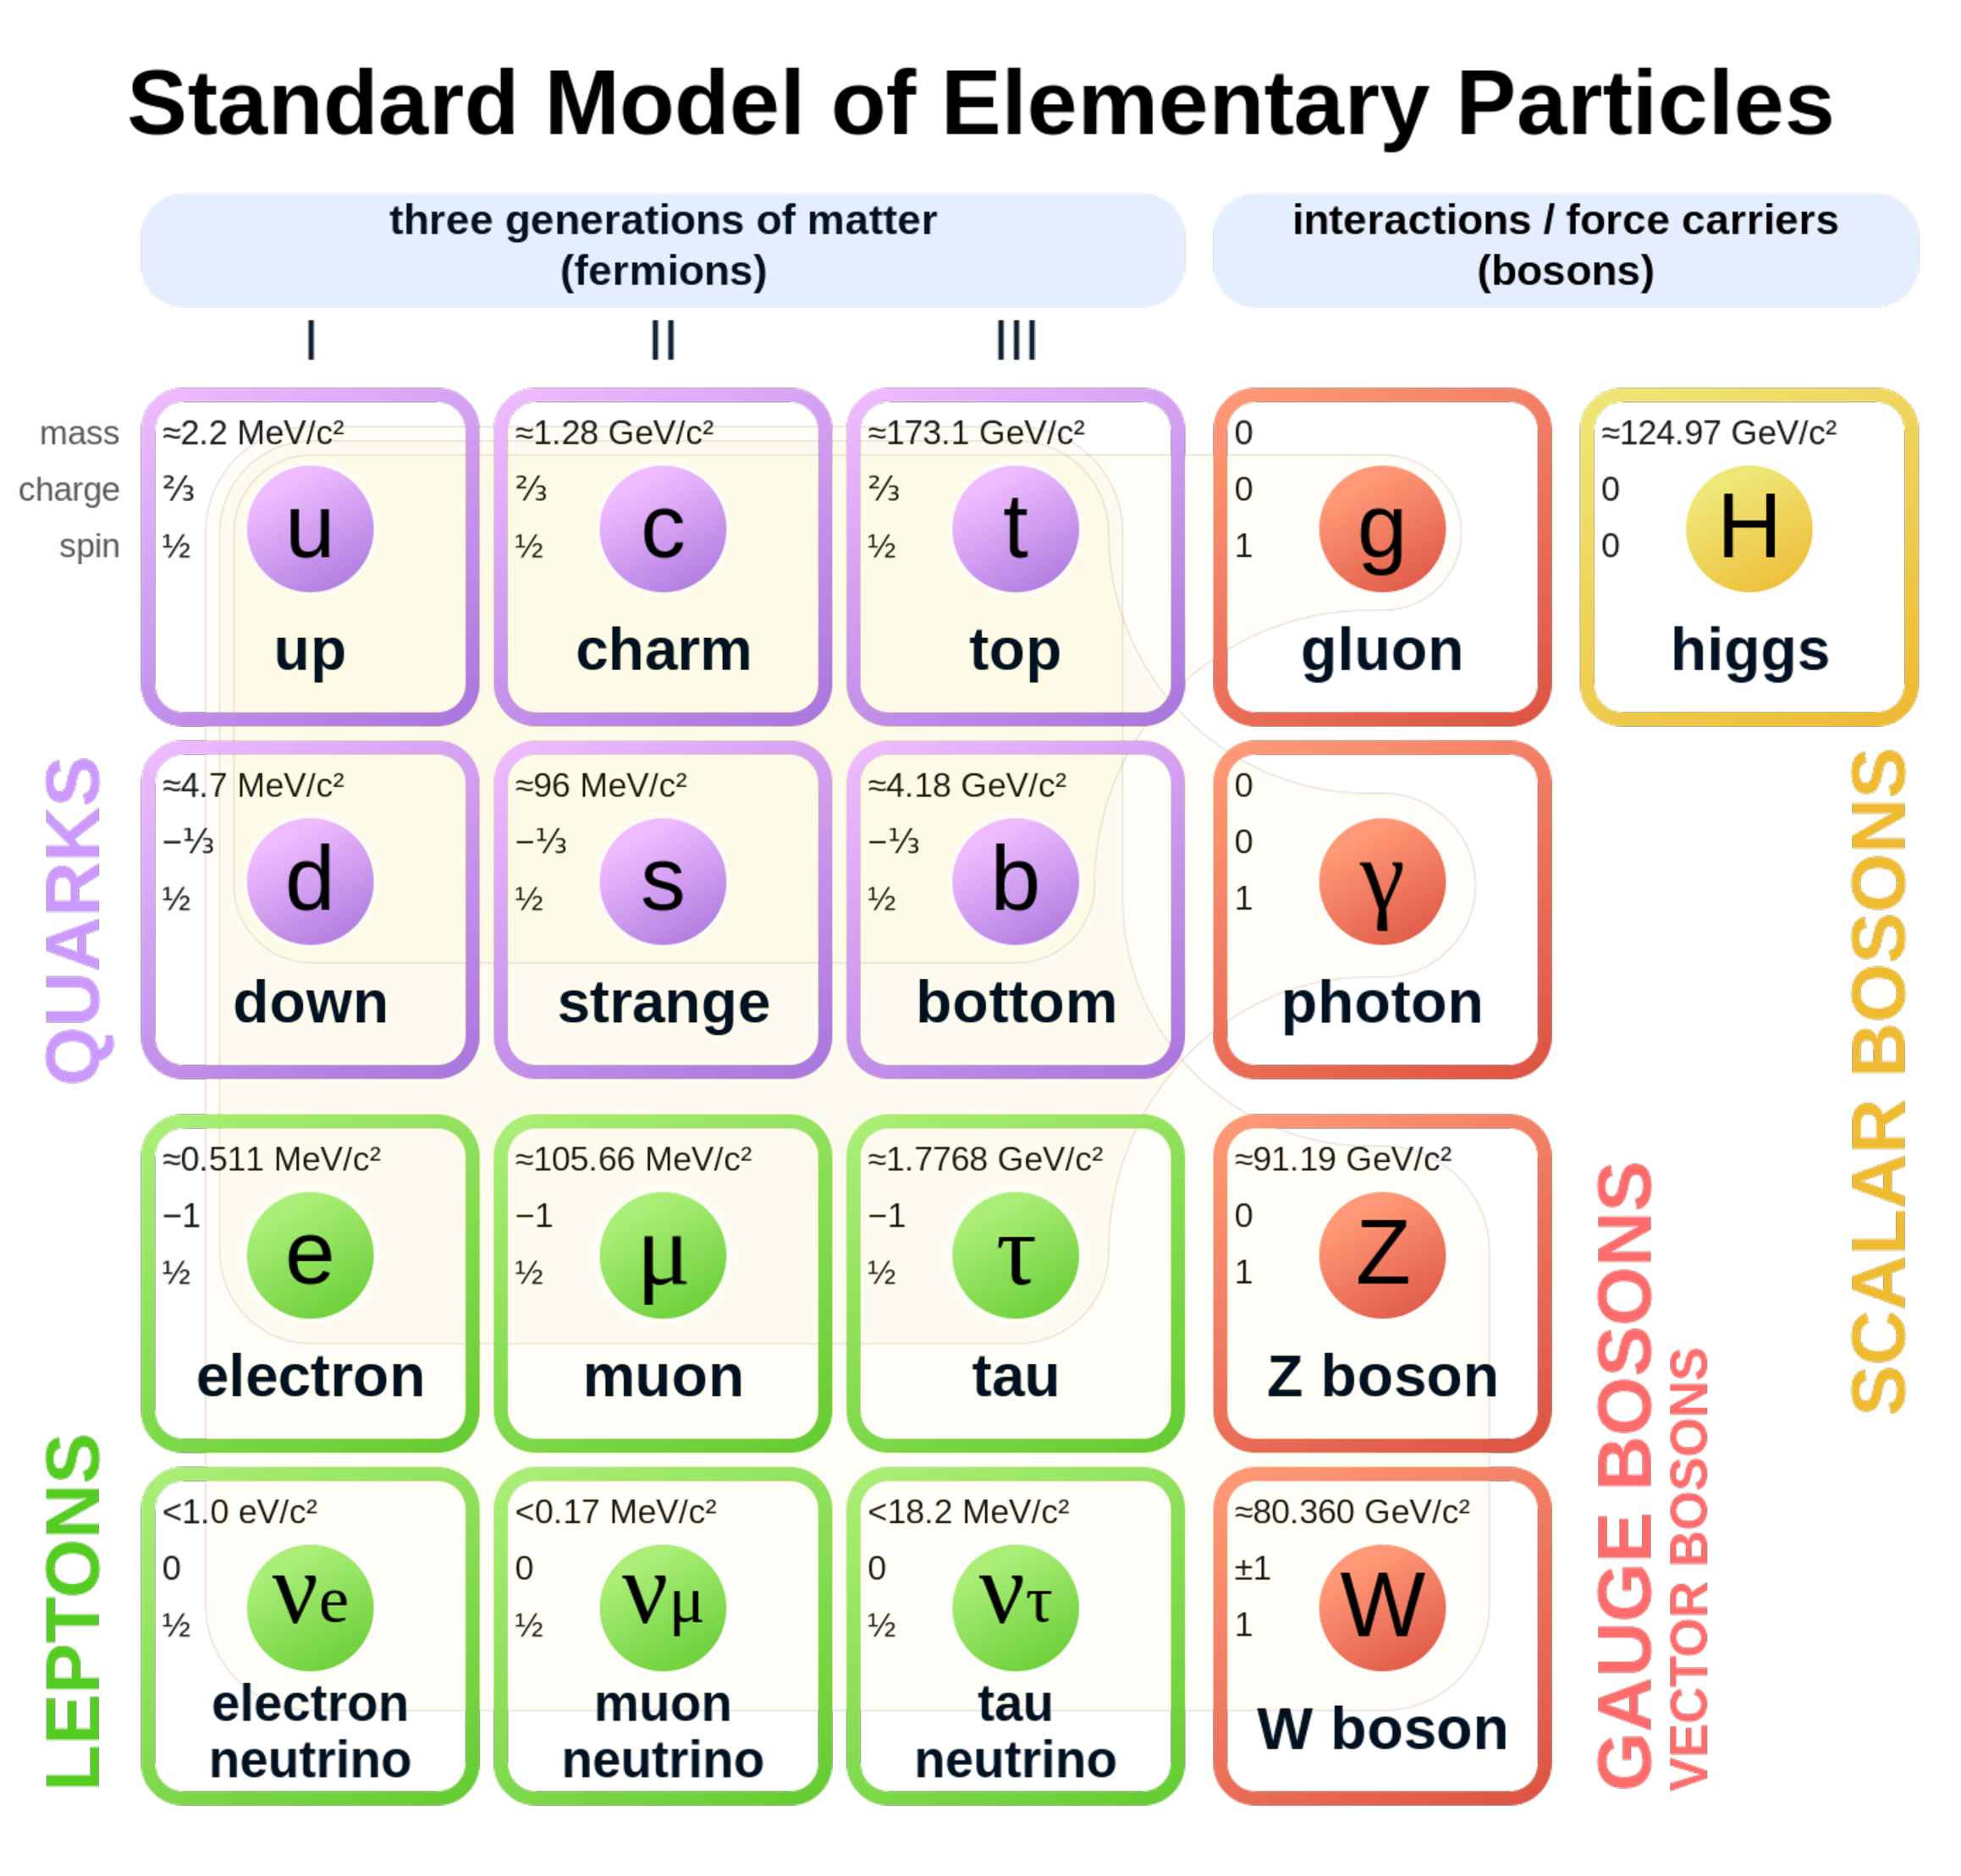
\includegraphics[width=0.9\textwidth]{figures/smParticles.pdf}
	\centering
	\caption{Fundamental particles within the standard model.}
	\label{fig:SM}
\end{figure}

\begin{figure}[htpb]
	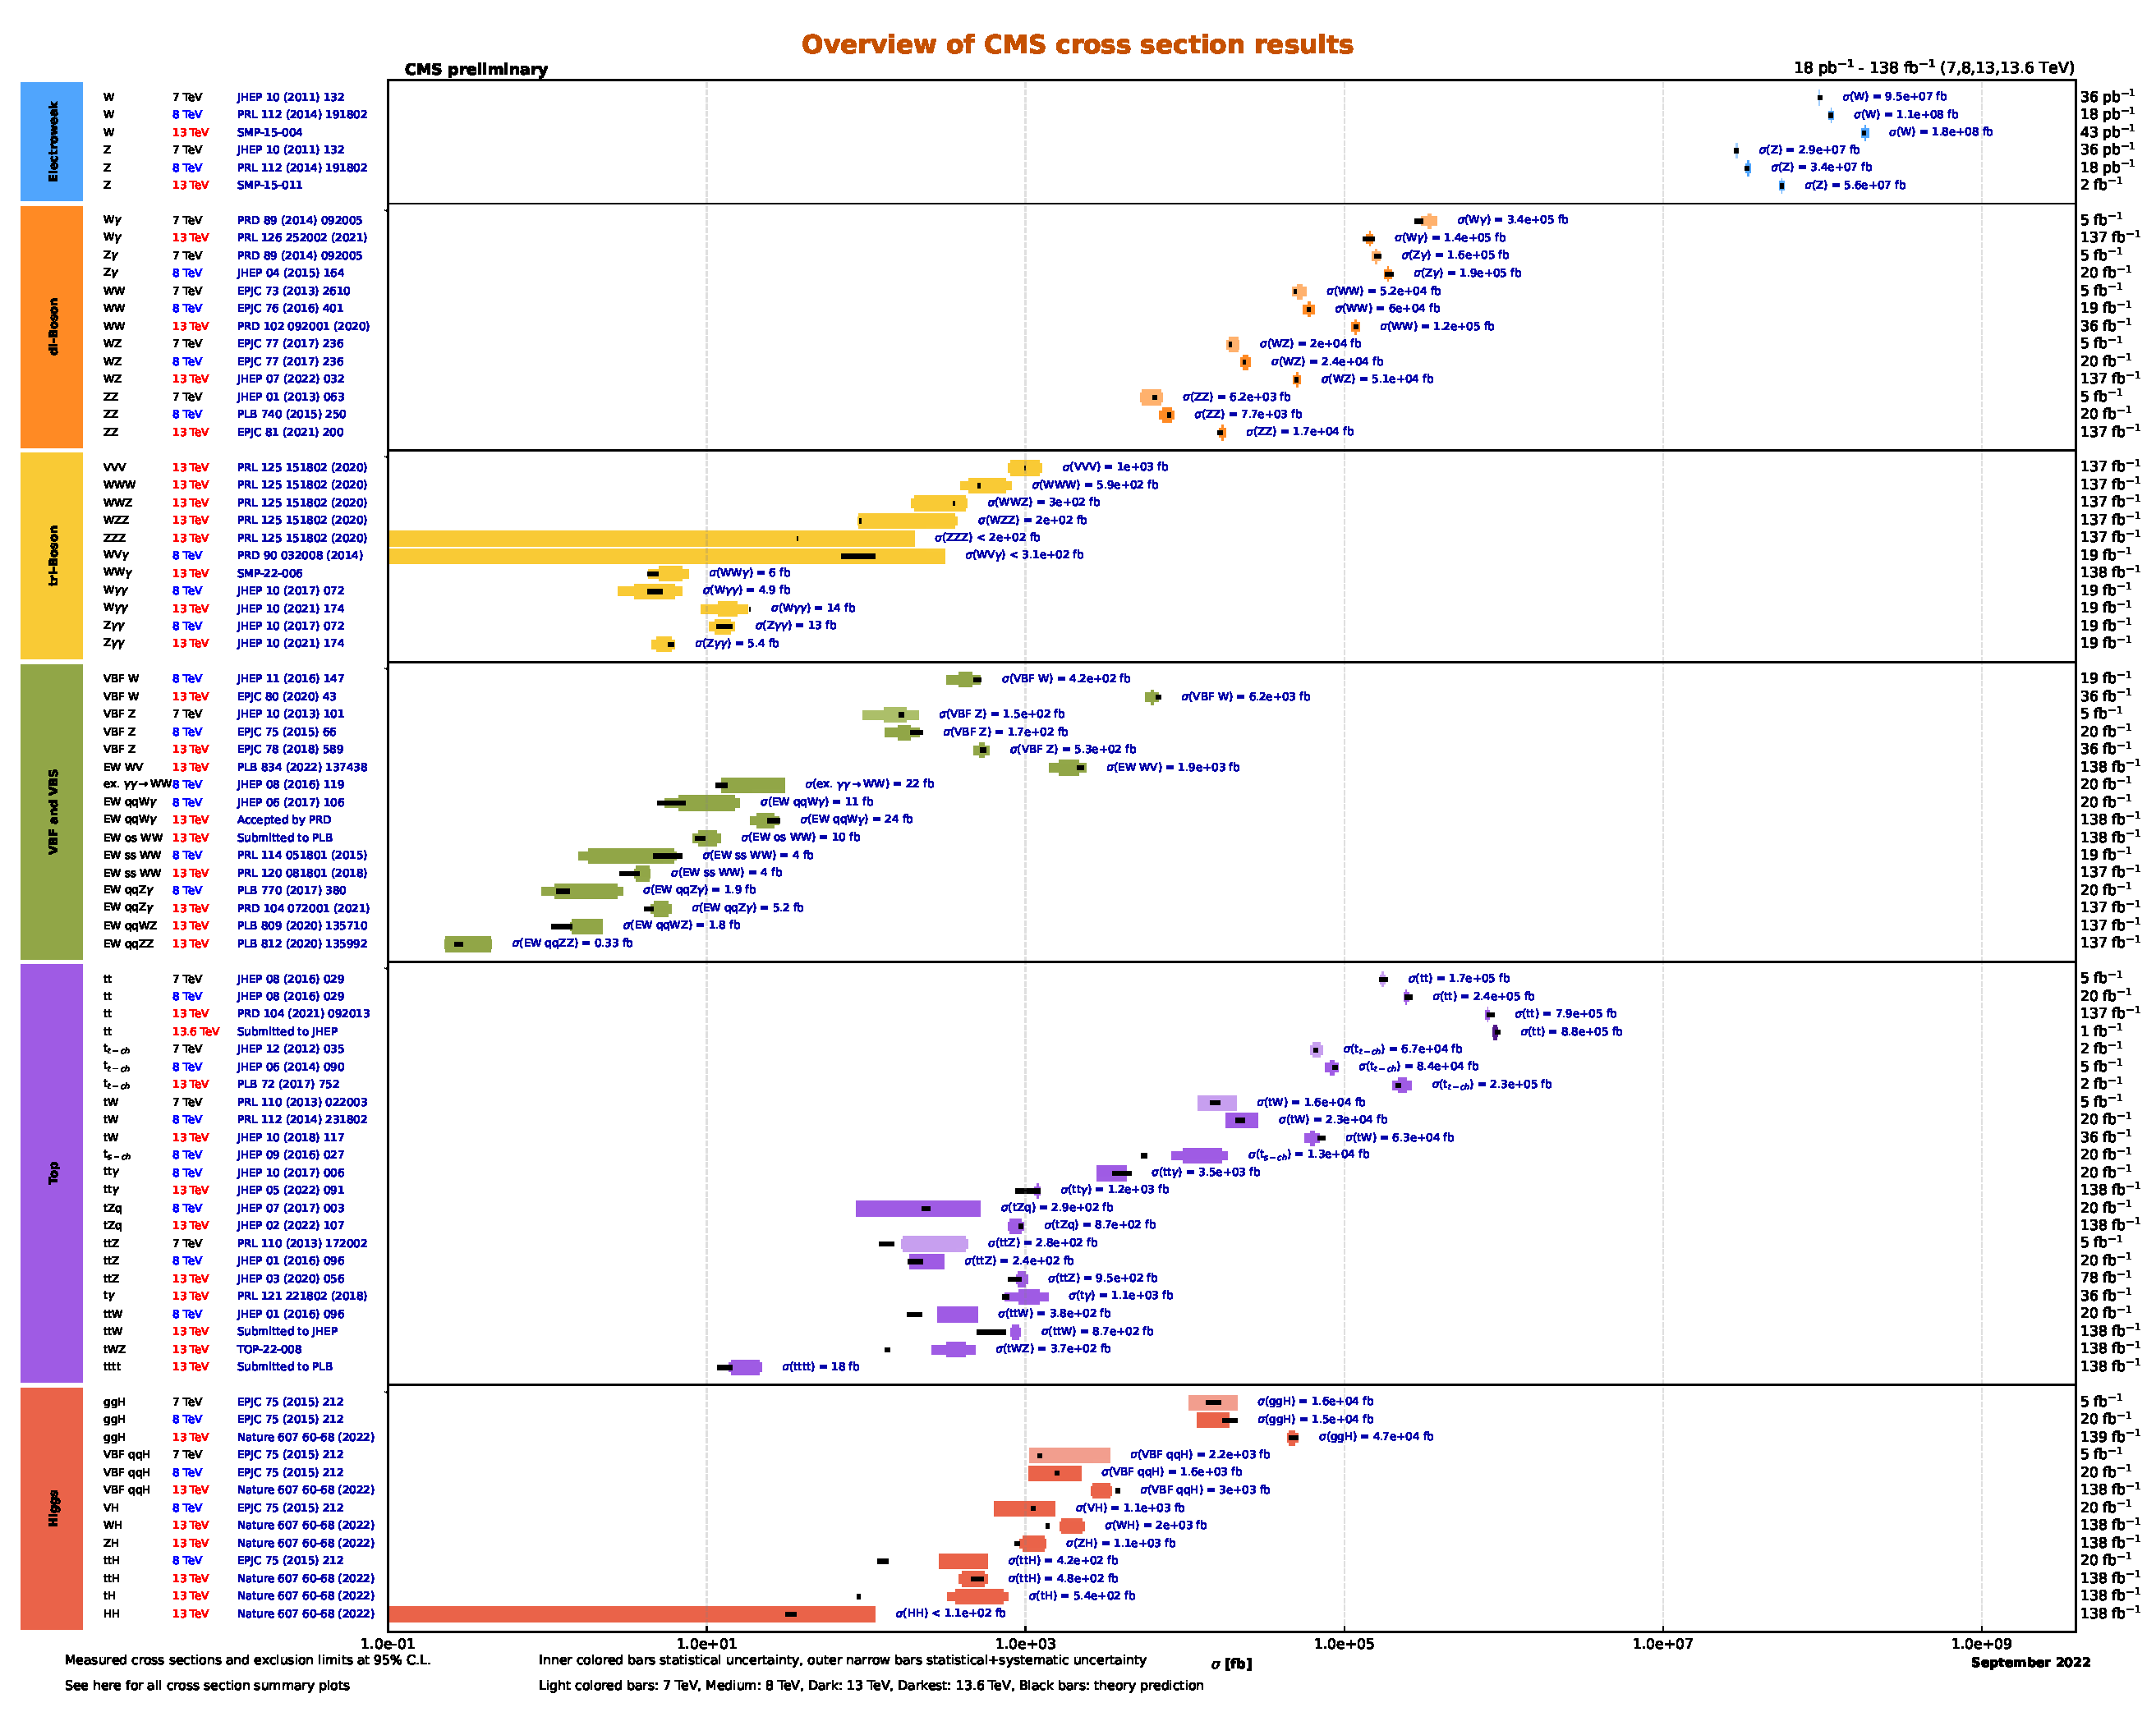
\includegraphics[width=0.9\textwidth]{figures/smRatePreds.pdf}
	\centering
	\caption[CMS Cross Section Results]{Predicted and measured cross sections over several sectors of CMS physics analyses. The predictions of the SM match the observed interaction rates to high precision over many orders of magnitude in cross section and a broad spectrum of processes.}
	\label{fig:SMratePreds}
\end{figure}

Developed over several decades through close collaboration between theory and experiment, the SM has been extremely successful at predicting a wide range of observed physics phenomena \Cref{fig:SMratePreds}.
Despite this success, there are several missing pieces in the SM such as gravity, neutrino masses, dark energy, and most significant to this paper, dark matter.
While these phenomena are observed in experiments, the lack of full information about the nature of the particles themselves or their interaction prevent their inclusion in the SM, and so keep it from being a complete description of all observed particle interactions.  

\section{Particulate Dark Matter}

%Graviational Lensing / Bullet Cluster
In addition to observations of excess mass in galaxies and nubulae from excess velocity in stellar motion, there are several other observations which indicate a particle origin for dark matter and constrain some aspects of its properties. 
While the velocities alone could be explained by alternate theories, such as non-luminous interstellar gas or modified newtonian dynamics, successful dark matter theories must address these additional astronomical observations as well. 

One of the best tools available to observe the dark matter distribution in the modern universe is gravitational lensing data \cite{Massey_2010}.
When photons pass through the warped spacetime of a gravitational field, their trajectories are deflected.
Massive objects, such as clusters of galaxies or dark matter, can create gravitational fields which deflect light rays analagously to a refracting lens.
When viewed from earth, light from distant objects can pass through these 'lenses' and be distorted or amplified, and through measuring this distortion the total mass required to produce it can be determined.

\begin{figure}
	\label{fig:gravLensing}
	\centering
	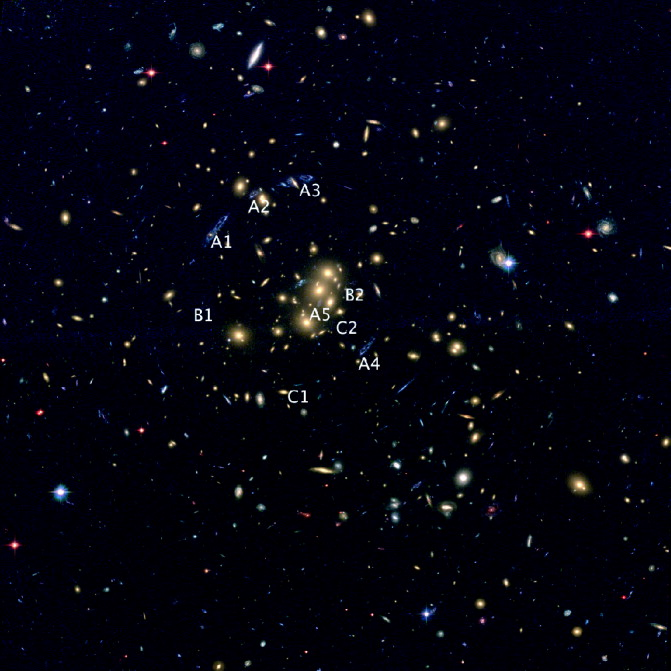
\includegraphics[width=0.4\textwidth]{figures/grav_lensing.jpg}
	\caption[Gravitational lensing of galaxy cluster CL0024+17]{ Color composite image of the galaxy cluster CL 0024+17. Ring-like distortions can be seen in projected images around the cluster due to lensing, as well as several cases where multiple images are formed from a single source. Five multiple images of a single magnified source are labeled as A1-5, while other potential candidates for multiple images are labelled as B1-B2 and C1-C2 \cite{jee2007}.}
\end{figure}

Gravitational lensing is traditionally split into 'strong' and 'weak' lensing regimes. 
In strong lensing, the space-time warping is strong enough for light to travel multiple paths along the lens and still reach the observer, resulting in light spreading into rings when lensed directly past a large mass, or potentially producing multiple images in lenses with complex shape.
Strong lensing can also occur in a 'microlensing' effect, where a source is directly along the line of sight to a star or other small object such that a lensing effect can be produced.
Because of the extremely small cross sectional area these stars that light must pass to produce microlensing, these events are typically observed transiently, as a background object passes directly behind a microlens and experiences a temporary magnification. 

In weak lensing, the light deflection is small, often appearing as local linear transformations of magnification, shear, and rotation. 
While difficult to measure directly, the images of multiple galaxies passing through the same dark matter halo will have identical shear transformations, producing correlations in their shapes.
By measuring these correlations over nominally uncorrelated galaxy shapes, the shear strength of this weak lensing can be statistically determined, allowing for measurements of dark matter distributions without requiring very high density.
Like traditional lenses, gravitational lenses are most effective when they are halfway between the source and observers on earth, though contributions from lensing along the entire path length impact the observed image.

Maps of the distribution of dark matter in the universe can be created by studying the lensing effect on light from distant galaxies which passes through dark matter clusters, even in cases where the luminous matter is insufficient to make direct velocity measurements, such as outer radii in galaxy halos beyond the range of the visible stars.
Lensing data produces many important observations for determining the properties of dark matter.
Using strong lensing data, the total mass of galaxy clusters can be measured, measuring the dark matter abundance to be roughly five times greater than luminous matter.
From microlensing data it can be determined that dark matter in our galaxy does not originate from free-floating, planet-sized non-luminous rock, as these 'free' planets would occasionally pass directly between earth and distant stars, causing temporary changes in brightness that have not been observed in microlensing surveys.

A particularly striking example of a particle dark matter comes from the bullet cluster, shown in \Cref{fig:bullet}. 
Galaxy clusters are formed from galaxies, interstellar gas, and dark matter.
In normal galaxy clusters these three constituents occupy the same general space and so their signatures are difficult to separate.
Unlike traditional clusters, the bullet cluster is formed from two galaxy clusters that collided around 150 million years ago. 
Because the galaxies and stars within the clusters are well spaced, their collision cross section was small, and most passed through without undergoing any collisions.
Unlike the galaxies, the interstellar gas in the clusters was uniformly spread and had a large interaction cross section causing it to be slowed by the collision, separating the gas from the main galaxy clusters and forming a shock front in the smaller of the two.

\begin{figure}[htpb]
	\label{fig:bullet}
	\centering
	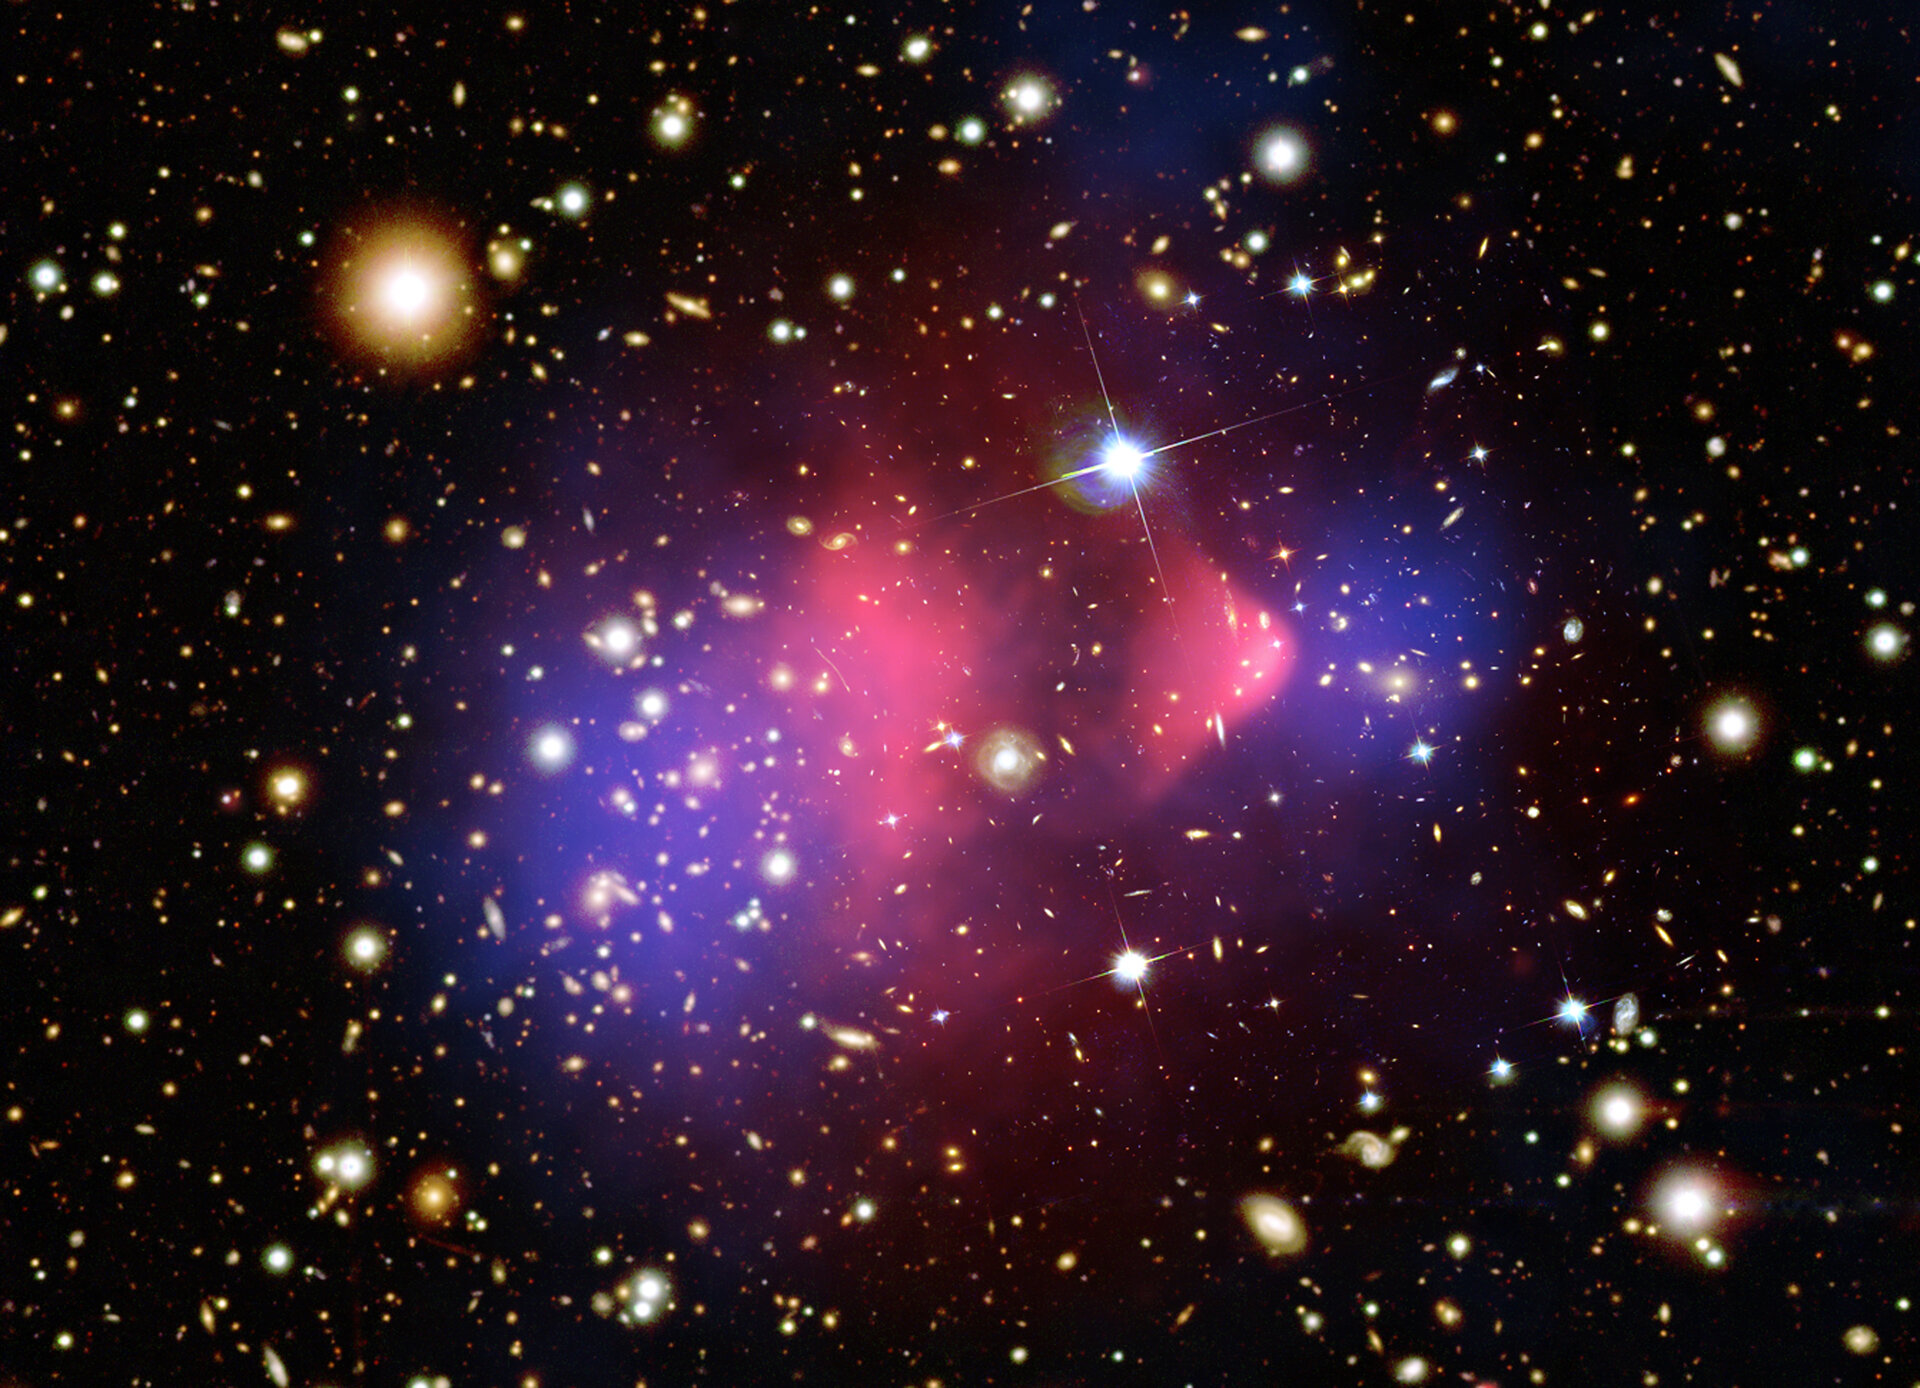
\includegraphics[width=0.8\textwidth]{figures/bullet_cluster.jpg}
	\caption[Visible, x-ray, and gravitational lensing images of the bullet cluster]{ A combined optical, gravitational, and x-ray image of the bullet cluster. Galaxies are shown in orange and white, while the x-ray image of the intracluster gas is in pink and the gravitational lensing data in blue. The mass distribution from lensing data is shown to remain with the galaxies and exhibit no signs of slowing from the collision, while the intracluster gas is greatly slowed and produces a collision shockwave in the smaller of the two clusters. X-ray: NASA/CXC/CfA/ M.Markevitch et al.; Lensing Map: NASA/STScI; ESO WFI; Magellan/U.Arizona/ D.Clowe et al. Optical image: NASA/STScI; Magellan/U.Arizona/D.Clowe et al.}
\end{figure}

By combining images of the cluster using visible light, showing the distribution of galaxies, x-ray emissions, produced from hot interstellar gas, and gravitational lensing, showing the total mass distribution, the behavior of each component during the collision can be seen. 
Crucially, the gravitational lensing data shows that the mass of the cluster lies with the main body of the stars while still representing a much larger mass than expected from only the luminous matter. 
This eliminates interstellar gasses of SM particles as a potential source of dark matter, and also provides constraints on the dark matter self interaction rate \cite{Randall_2008}, as the two diffuse dark matter halos passed through each other without discernable drag from collisions.

%Cosmic Microwave Background
Some of the most detailed measurements of the relative abundance of dark matter come from observations of the cosmic microwave background (CMB).
The CMB is radiation which originated in the early universe, when SM matter consisted of hydrogen and helium plasma and free electrons.
Because of scattering with these free electrons, the universe was opaque on cosmological scales until the plasma cooled and was converted into a gas. 
At this point, thermal radiation from the plasma could travel through the universe without significant scattering probability, and these photons can be observed today as the CMB, constant microwave radiation that is visible from every direction (\Cref{fig:CMB}).

\begin{figure}[htpb]
	\label{fig:CMB}
	\centering
	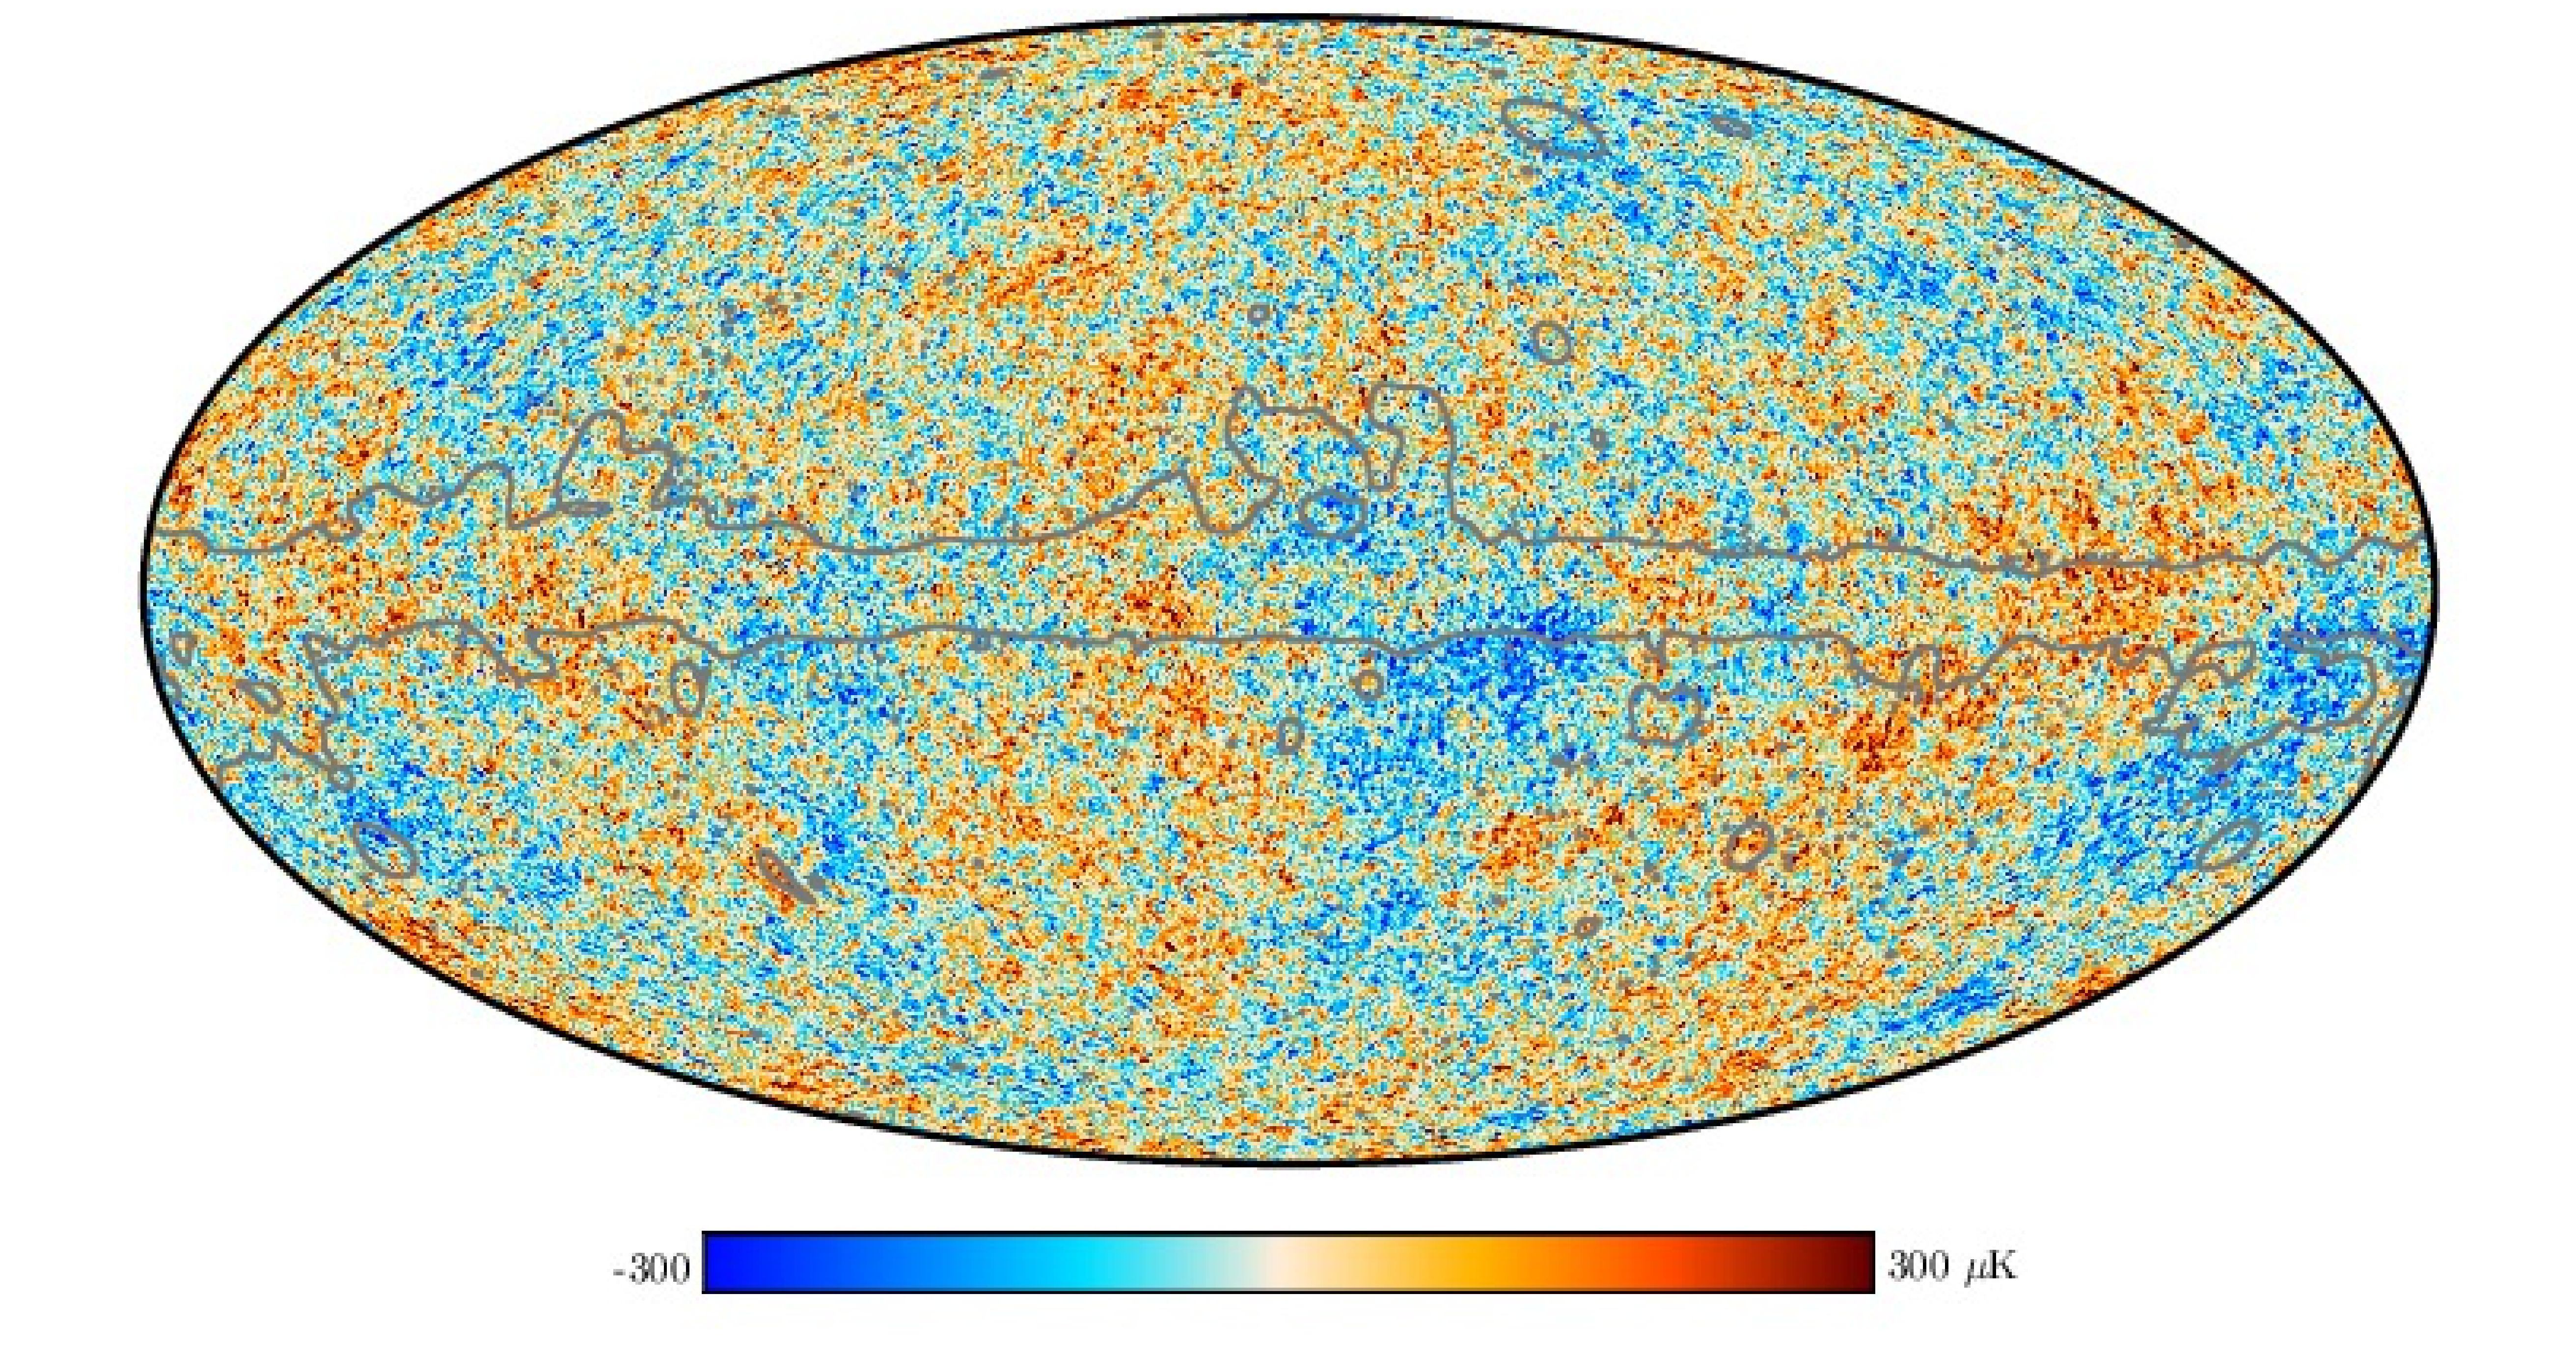
\includegraphics[width=1.1\textwidth]{figures/cmb.png}
	\caption[The CMB temperature anisotropy]{The temperature anisotropy of the CMB. Outlined in gray are regions of high microwave background, primarily aligned with the main body of the milky way, which are treated specially to reduce their backgrounds \cite{PlanckCMB}.}
\end{figure}

The conversion of primordial plasma into a hydrogen and helium gas occurred when the universe was roughly 400,000 years old, and the CMB therefore provides an image of its temperature and density distribution at that time.
While the primordial plasma was nearly homogeneous, there were slight variations of order one part in ten thousand, which later grew by gravitational attraction and led to the formation of galaxies and stars \cite{kurkisuonio}.
By studying these anisotropies, the dynamics of the baryon-photon plasma can be inferred, and several properties of early cosmology, including the mass density of dark matter, can be determined.

The anisotropy of the CMB is measured through correlations in the temperature of different points as a function of the length scale between them. 
As the CMB forms a 'sphere' of the observable sky, these distance are expressed as length scales, and it is convienient to analyze them as expansions of spherical harmonics, which can be shown to only depend on the order of the angular scale parameter $l$. 
By measuring the pertubation of the CMB and decomposing it into sperical harmonics, the angular power spectrum can be measured \Cref{fig:CMBpowerSpectrum}, from which details about the composition of the early universe can be inferred.

The angular power spectrum of the CMB consists of a series of peaks of decreasing amplitude with increasing multiple moments. 
At large scales, $\theta >> $\ang{1}, the distances between spatial points are larger than the Hubble distance between them, and therefore cannot have any dynamic evolution in the primordial plasma.
At smaller scales, $\theta < $\ang{1}, the perturbations are close enough to communicate before the plasma condenses, and so can show evidence of plasma dynamics.

\begin{figure}[htpb]
	\label{fig:CMBpowerSpectrum}
	\centering
	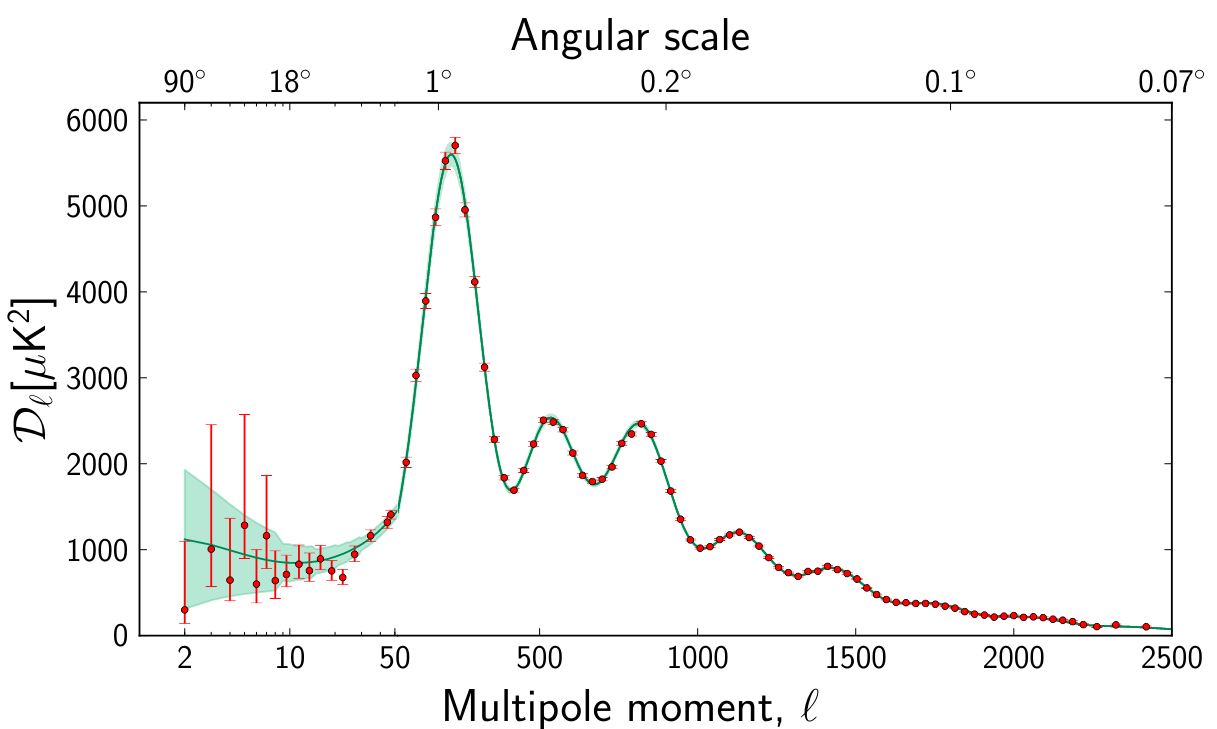
\includegraphics[width=0.8\textwidth]{figures/cmb_power_spectrum.png}
	\caption[The temperature angular power spectrum of the CMB]{The temperature angular power spectrum of the CMB. The points correspond to measured data from the Planck satellite, while the line is formed from a best-fit to a six-parameter cold dark matter model \cite{PlanckCMB}.}
\end{figure}

Initially, anisotopies are present from quantum fluctuations which expanded to cosmological scales during inflation.
Regions with increased densities then attract the photon-baryon fluid gravitationally, amplifying the flucutation.
This increased density then causes a corresponding increase in the temperature of these regions and thus their radiation pressure, which eventually overcomes the gravitational attraction and begins to push the fluid out of the region. 
This pattern of gravitational and radiation driven motion form acoustic oscillations with Fourier modes that oscillate at frequencies dependant on the sound speed in the baryon-photon fluid.

The expansion of the universe causes the sound speed and plasma density to change with time, with the notable effect that the perturbation amplitude is maximal at angular scales which are at their extrema when the photons decoupled. 
This produces the peak structure seen in the CMB power spectra, with each maximum corresponding to an acoustic mode with frequency which happened to be at a maximum during the time of decoupling.

Beyond solely acoustic oscillations, this pattern is also strongly impacted by the presence of dark matter.
Initially distributed similarly to the photon-baryon plasma, dark matter will also be drawn into gravitational wells caused by regions of increased density produced by quantum flucutations before inflation.
Unlike SM matter, dark matter has very little or no radiation pressure, and thus will not directly undergo acoustic oscillations with the plasma. 
Only interacting via gravitational potential, dark matter follows the plasma into the gravitational wells but not leaving from the radiation pressure. 

Due to this interaction difference, the presence of dark matter significantly changes the oscillation frequency and the relative amplitude of each acoustic peak.
The angular power spectrum can thus be fit with a seven parameter cold dark matter model and produce strong constraints on the abundance of dark matter.
Through these fits, the mass density of dark matter in the universe is determined to be \SI{4.1e-27}{\kilo\gram\per\meter\squared} \cite{PlanckCMB}, roughly 5 times more than the total abundance of SM matter.

%Structure Formation
Through these cycles of gravitational compression and radiation-pressure driven expansion, dark matter tends to be collected into nodes and filaments of increased mass. 
These collections of dark matter have profound impacts on structure formation in the universe after the plasma combines into gas.
By providing centers of gravitational attraction, the dark matter clusters greatly increase the rate at which stars and galaxies form.

In models constructed using only gas from the condensed plasma with mass anisotropy matching the known distribution of the CMB, star formation occurs at much longer timescales than models which include dark matter.
Because of these longer timescales, the resulting distribution of the simulated modern universe shows much greater uniformity than is observed today. 
By using information from weak lensing, the current structure of dark matter halos can be measured, and compared with various simulations of structure formation to test the validity of different dark matter models.

In addition to the total mass and initial distribution of dark matter, these models also provide information on the possible temperature of dark matter.
Cold dark matter models, where dark matter decouples from SM matter at lower temperatures, , the lower relative velocity allows the gravitational attraction to dominate dark matter dynamics, forming clusters similar to those observed today.
In models with higher temperature dark matter the thermal motion plays a much larger role, resulting in chaotic waves of dark matter which do not form these clusters and can destroy structure in SM matter when they pass near it and disrupt the gravitational wells.

%Baryogenesis
An additional observation indicating that dark matter cannot be explained by standard model matter comes from simulations of big-bang nucleosynthesis. 
In the first few minutes after the big bang, hydrogen, helium, deuterium, and lithium are produced from the quark-gluon plasma. 
The relative production of these light elements depends on the total Baryon density during nucleosynthesis, and thus can be used to determine the total density of baryons in the early universe (\Cref{fig:baryogenesis}).

\begin{figure}[htpb]
	\label{fig:baryogenesis}
	\centering
	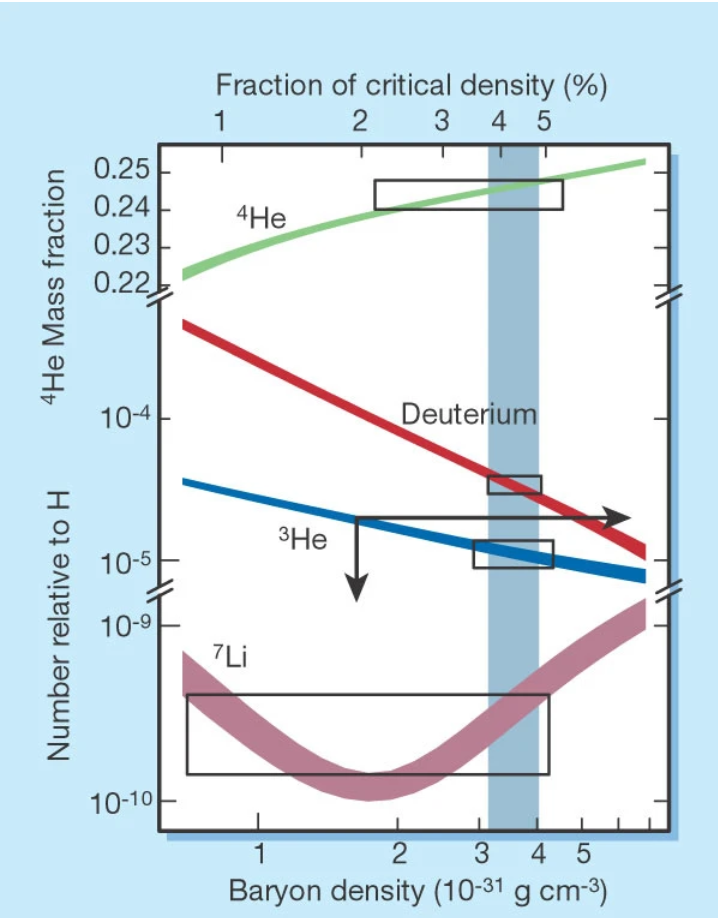
\includegraphics[width=0.6\textwidth]{figures/baryogenesis.png}
	\caption[Relative Light Baryon Abundancies]{The relative abundancies of primordial nuclei as a function of the total baryon density and the 'critical' density, the matter density requred to produce the observed flat curvature of the universe. The boxes represent observed estimates of the primordial abundancies, and the shaded blue region the range of densities determined from deuterium, the most precisely measured of the abundancies. Figure from \cite{charbonnel2002}.}
\end{figure}

Direct observations of the baryon density have large uncertainties due to the significant fraction of non-luminous matter contained in interstellar gas, but using this method precise measurements can be made without relying on estimations of the proportion of luminous to non-luminous matter.
Comparing this measurement of the total baryon density in the universe to the total mass density observed from cosmological observations, it is seen that the baryon density is roughly 4\% of the total \cite{Tytler_2000}, indicating that a very significant portion of the total mass density in the universe must originate from some beyond the standard model source.

\section{Thermal Dark Matter}
While a particulate explanation of dark matter is well motivated, very little can be concluded about its properties, and a very wide range of potential models can be searched for in experiments.
To help identify dark matter signatures that may be visible in a detector based experiment, several assumptions are be made relating to its nature, the first being a thermal origin for dark matter.

The core assumption of thermal dark matter models is that the interaction between dark matter and SM matter is significant enough that for some period of time in the early universe dark matter was in thermal equilibrium with standard model matter.
This allows dark matter to be produced simultaneously with SM matter during the universe's inception rather than as a separate process, and also requires that dark matter have some coupling to SM matter, which would also be necessary for its observation in an experiment like CMS.

This thermal equilibrium is achieved to due the high temperature and density of the early universe where, despite small SM couplings, dark matter particles can be frequently produced through interactions with standard model particles and produce standard model particles through their own interactions and decays.
As the universe expands and cools, the relatively large mediator mass causes the production of dark matter from collisions of SM particles to cease, thermally decoupling SM matter from dark matter.
After dark matter production ceases, its annihilation continues for some time until the expansion of the universe causes the density to fall, reducing the interaction rate below the Hubble expansion rate so that dark matter "freezes out", leaving a fixed number density of dark matter with its phase-space distribution subject only to the universe expansion and eventual structure formation \cite{thermalDM} (\Cref{fig:freezeout}).

\begin{figure}
	\label{fig:freezeout}
	\centering
	%\includegraphics[width=0.5\textwidth]{figures/freezeout.png}
	\caption[Thermal Freeze-Out]{A thermal freeze-out model for some stable species. At early times, the particle is in thermal equilibrium with SM matter and has a constant density. As time progresses, the production ceases while annihilation continues, resulting in a continuously decreasing density. Eventually, the production probability becomes small enough that the particle annihilation also ceases leaving behind a constant relic abundance, with density related to the interaction cross section and mean particle velocity. Figure from \cite{hooper2009tasi}.}
\end{figure}

For any given thermal dark matter model a 'relic target' cross section can be calculated - the cross section required to produce the density of dark matter seen today.
For any given dark matter coupling strength and particle mass, the thermal relic model will set a specific freeze-out temperature and number density.
By combining this number density with the observed astronomical mass density, the coupling strength can be related directly to a dark matter mass, with heavier particles requiring lower number densities and therefore later freeze-out temperatures and larger interaction cross sections.

\section{Light Dark Matter}
Traditional searches for thermal dark matter have tended to focus on models which interact via the nuclear weak force, which have relatively larger dark matter mass requirements (M$>\sim$few GeV), and so are easier to observe with indirect detection experiments searching for collisions of halo dark matter particles with passive detectors.
While this larger mediator mass, weakly interacting phase space is well-covered from a wide variety of experiments, dark matter could also be explained using mediators in a 'light' mass region, ~MeV to ~GeV, which act as a 'portal' to couple dark sector particles to the SM \cite{darkSectors}.

A simple renormalizable interaction which can be introduced to the SM which could create this light coupling is a kinetic mixing between a new gauge boson with field strength $F'_{\mu\nu}$ and the hypercharge field $B^{\mu\nu}$ through the operator $\mathcal{L}$ (\Cref{eq:LDMlagrangian}). 

\begin{equation}
	\label{eq:LDMlagrangian}
	\mathcal{L} = - \frac{\epsilon}{2} B^{\mu\nu}F'_{\mu\nu}
\end{equation}

For small mixing parameter $\epsilon$ and light gauge bosons, these new couplings align with those of the SM photon \cite{Bauer_2018} and so this new gauge boson is referred to as the "dark photon", or A'.
Through these couplings, any SM process which produces a photon could instead produce a dark photon, with suppression proportional to the mixing parameter.

This coupling represents the minimal kinetic mixing, encoding the kinetic coupling as a free parameter instead of arising from specific interactions within a chosen theory. 
While technically forming a dark sector on its own, this model must be extended with additional particles to act as dark matter candidates, as models with only dark photons would cause them to decay back into SM particles.
These dark matter candidates would couple to the dark photon via dark-sector gauge interactions with some coupling strength $g_D$, and can be either fermions or scalar bosons.
As these dark sector particles are assumed to not leave visible signatures within our detector, their influence in this search is limited to setting the branching fraction of the dark photon decaying to either visible SM particles or 'invisible' dark matter.
As this search focuses on these invisible dark photon signatures, it is assumed that $g_D$ is much larger than $\epsilon$ and that the mass of the dark matter candidates is less than twice the A' mass such that they will decay dominantly to dark matter particles or have significantly long lifetimes to pass out of the detector acceptance.


\section{Targeting Dark Matter Production}
If a light dark matter coupling were present, there are several potential signatures that could appear in an experiment like CMS.
Traditional searches in CMS look for particle production in the initial scattering process between proton constituents.
As a light dark matter coupling would allow mixing between the \aprime and any standard model photon, dark matter could be produced in initial state collisions with electromagnetic interactions between partons that produce photons that then mix with the \aprime.

Unfortunately, decays of the \aprime outside of the detector or into other dark matter particles which are invisible to CMS make this initial production mode very difficult to distinguish.
Events with large initial state radiation from the partons can make this signal visible as a large missing transverse momentum in the event, but the large reduction in acceptance from this type of requirement causes the resulting limit to be very weak.

Instead of searching for dark matter production in the initial state, the signal could appear in a secondary interaction between a final state particle and the detector itself.
The relatively small masses of light dark matter particles limits the loss in the interaction rate due to the much lower center of mass energy in these secondary interactions compared to the initial collision, and the high particle flux and large size of the detector result in a significant fixed target luminosity.

The primary signature of a secondary interactions between a particle emitted from the initial collision and the detector would be missing energy carried by the invisible \aprime and a change in the trajectory of the visible particle.
These types of signatures are difficult to observe in particles with large standard model interaction rates, as the shower of particles produced in their interactions can lead to large uncertainties in their energy measurement and little hope of observing trajectory differences.
In addition, high interaction rates expose particles to less of the detector as they are stopped relatively quickly, reducing the effective luminosity.

For these reasons, the selections in this search focus on potential dark matter interactions of final state muons.
As muons have small standard model cross sections they lose very little energy while they traverse the detector, leading to high consistency in projecting their trajectory and observing potential changes, as well as low rates of stopped muons due to standard model processes which could fake the energy loss to an \aprime.

With a light dark matter mixing, muons would primarily produce dark matter in the mass ranges of interest via a process known as \dbrem, where a dark matter particle is emitted from a muon as it recoils from the electromagnetic field of a nucleus in the detector (\Cref{fig:dbrem_feyn}).
While other processes, such as photoproduction of vector mesons which then decay invisibly through dark matter coupling, would also be present with the assumed coupling, only \dbrem is considered in this search due to its significantly larger production rate.

\begin{figure}[ht]
	\centering
	\label{fig:dbrem_feyn}
	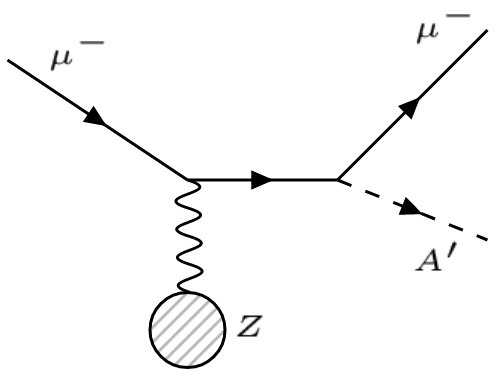
\includegraphics[width=0.8\textwidth]{figures/dbrem_feyn_diagram.jpg}
        \caption[Dark Bremsstrahlung Feynman Diagram]{Dark Bremsstrahlung caused by a muon interacting with a nucleus with atomic number Z.}
\end{figure}

As an additional feature of muon-initiated \dbrem, results from this search are also sensitive to dark matter models which replace the generic dark matter mixing with an asymmetric coupling to the lepton generations.
While lepton universality is built into the standard model, no such requirement is necessary for new physics models. 
Instead of the fully generic kinetic mixing presented in \Cref{eq:LDMlagrangian}, the dark photon gauge field can be chosen to contain an additional current which carries charge proportional to muon number minus tau number, ($L_\mu - L_\tau$) \cite{neut_trident}.
This type of field would result in a dark matter coupling that preferentially interacts with muons and taus, and has few existing constraints as it only would affect neutrinos and unstable leptons.

There are several experimental anomalies which could potentially be explained by an asymmetric lepton coupling of this type.
The measurement of the muon magnetic moment by the Fermilab E989 experiment \cite{gminus2}, combined with the original result from Brookhaven \cite{gminus2_bnl} leads to a 4.2 $\sigma$ discrepancy with the theoretical prediction \cite{gminus2_theory}. 
This could potentially be explained by a dark matter signal which preferentially couples to muons, as the dark matter coupling would alter the muon magnetic moment through additional loop diagrams.
A muon-philic cross section would also have a larger thermal relic cross section, as requiring a muon or tau coupling in its production reduces the available paths in its creation and so requires increasing the remaining cross section to achieve the same freeze-out number density.

\section{Z-Bosons and the DY Process}
For muons to potentially interact within the CMS detector and produce dark photons, they must first be created within the initial collision.
Many processes in CMS collisions can produce outgoing muons, but while accepting muons from any process would allow for very high signal rate the difficulty of identifying a muon using only inner detector information (see \Cref{sec:muonReco}) would result in large contributions from backgrounds where the reconstructed particle does not originate from a real muon.
To help control these backgrounds, muons from particle resonances can be selected, where neutral particles created in the hard scatter between the initial state quarks produce oppositely-charged pairs of muons.
When di-muon pairs are produced via mediator particles, the invariant mass spectrum of the produced particles peaks sharply near the mediator particle mass, with the peak width proportional to the lifetime of the mediator. 
By selecting muons from particle resonances, one outgoing muon can be used to 'tag' the event, and the other can be used to 'probe' the response of the detector along its trajectory to search for non-standard interactions. 

While many such resonances exist in the CMS di-muon spectrum (\Cref{fig:diMuonSpectrum}), this search targets muon originating the decay of Z bosons due to the relatively higher energy of the produced final-state muons and the reduced rates of non-resonant muon pairs near the Z mass.
Z bosons are the neutral carrier of the nuclear weak force, which unlike the electromagnetic and nuclear strong forces has massive force carrying bosons.
Specifically, the Z boson mass is near \SI{90}{\giga\eV}, 
Z bosons will decay into dilepton pairs with nearly equal rates between electrons, muons, and tau leptons. 

\begin{figure}[ht]
	\centering
	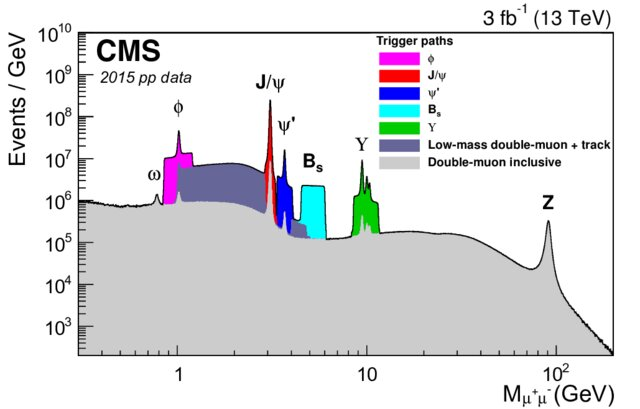
\includegraphics[width=\textwidth]{figures/cms_diMuonSpectrum.jpg}
	\caption[Inclusive dimuon spectrum in CMS]{The dimuon invariant mass spectrum in the CMS high-level trigger, measured using data collected in 2015. Figure from \cite{cmsMuonPerformance}.}
	\label{fig:diMuonSpectrum}
\end{figure}

The Z boson resonance in di-muon pairs is primarily produced through the Drell-Yan (DY) process \cite{origDYPaper,DYSummary}, in which a pair of quarks in the initial hadron collision annihilate into a pair of leptons (\Cref{fig:dyDiagram}).
The invariant mass of di-muon pairs produced in the DY process with minimal selection requirements is shown in \Cref{fig:dySpectrum}, as well as the energy of the individual muons produced. 

\begin{figure}[ht]
	\centering
	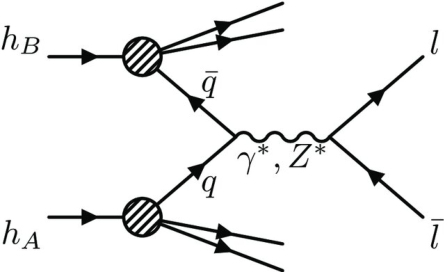
\includegraphics[width=0.45\textwidth]{figures/dyProcess.pdf}
	\caption[Feynman Diagram for the DY Process]{The Drell-Yan process. A quark from one hadron annihilates with an anti-quark from another, resulting in the production of two leptons. Figure from \cite{bechtel2023}.}
	\label{fig:dyDiagram}
\end{figure}

\begin{figure}[ht]
	\centering
	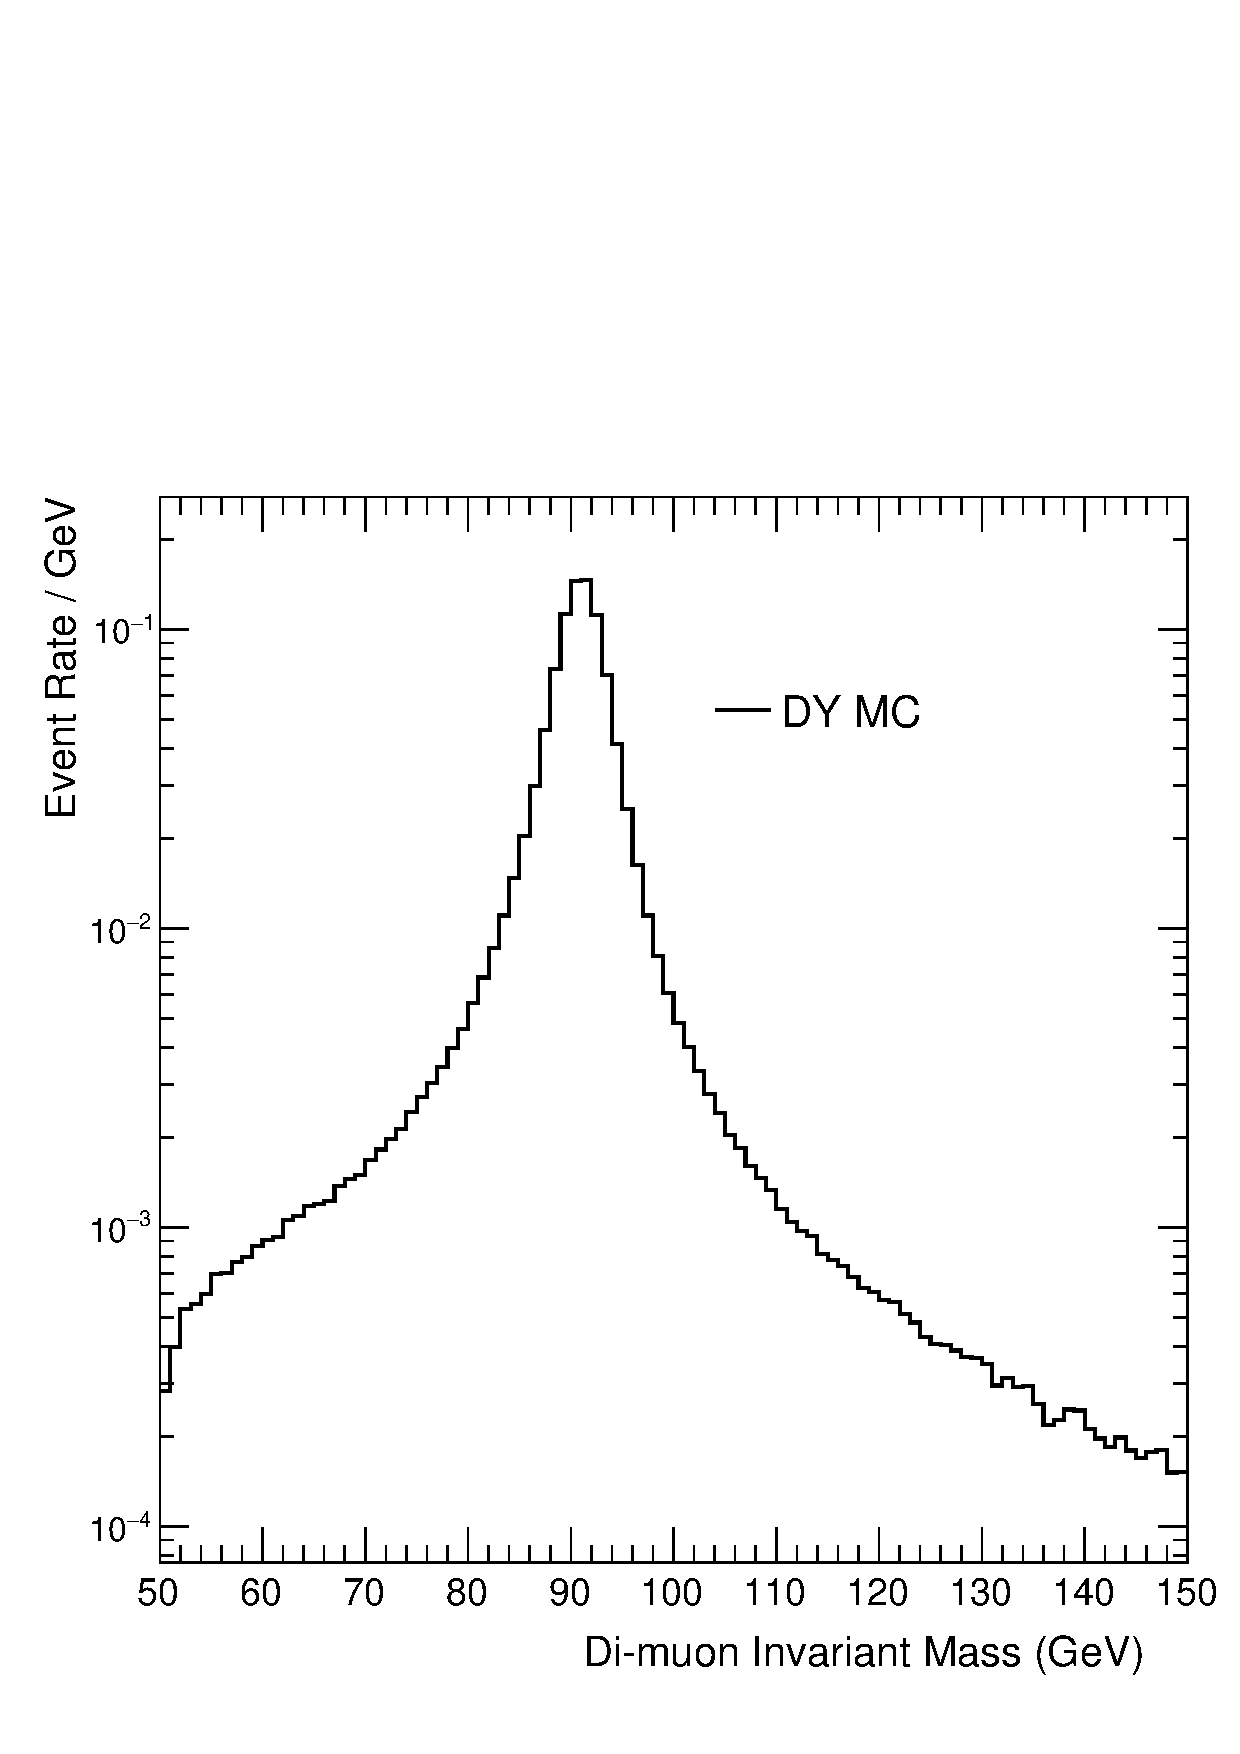
\includegraphics[width=0.45\textwidth]{figures/dyMuSpectrum.pdf}
	\hspace{0.01\textwidth}
	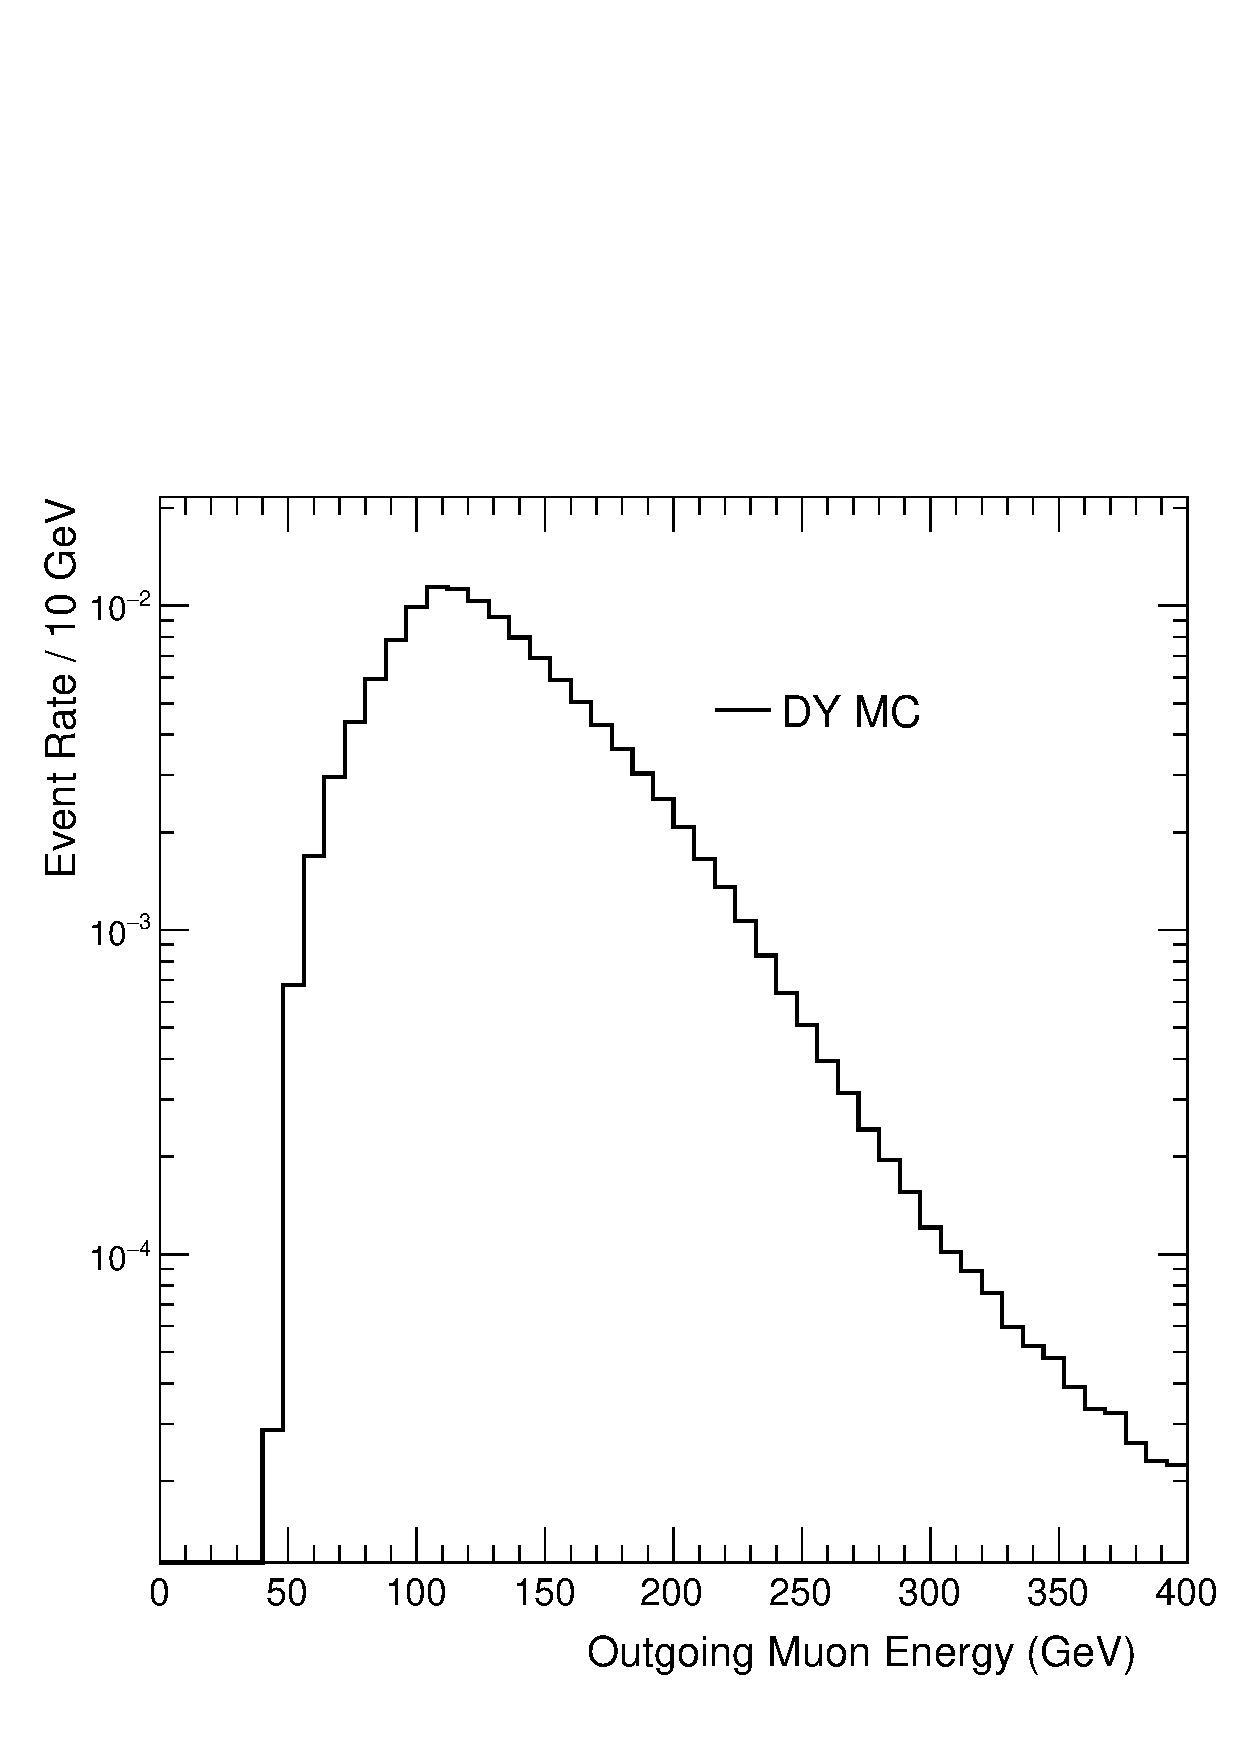
\includegraphics[width=0.45\textwidth]{figures/dyMuEnergy.pdf}
	\caption[DY Process Di-muon Invariant Mass and Outgoing Muon Energy]{The simulated di-muon invariant mass spectrum for DY events in CMS with minimal selection criteria (left), and the corresponding energy of the outgoing muons (right).}
	\label{fig:dySpectrum}
\end{figure}


%%%%%%%%%%%%%%%%%%%%%%%%%%%%%%%%%%%%%%%%%%%%%%%%%%%%%%%%%%%%%%%%%%%%%%%%%%%%%%%%
